\documentclass[a4paper,10pt]{article}
\usepackage[utf8]{inputenc}
\usepackage{graphicx}
\usepackage[sf, bf]{caption}

\setlength{\parindent}{1em}

\begin{document}
    \huge 
    \noindent
    \textbf{Brunn User Documentation}

    \normalsize

    \section{The main window in Bioclipse}
        First a few general words about how Bioclipse works.

        \subsection{Editors and Views}
            Bioclipse is made up of editors and views. Editors are for editing
            things. Items can be opened in an editor, edited and then saved and
            the editor closed. A view can listen to, and change appearence
            according to, what is selected. For example the properties view
            shows the properties of the item currently selected. Figure
            \ref{editorsAndViews} shows an example of what are views and what
            are editors in a standard Brunn window.
            
            \begin{figure}[htbp]
                \begin{center}
                    \includegraphics[width=1\textwidth]{images/EditorsViews.png}
                \end{center}
                \caption{\textit{The Bioclipse workspace consists of editors
                                 and views. The editors are stacked in the
                                 middle and the views can be moved around.}}
                \label{editorsAndViews}
            \end{figure}

        \subsection{Two ``hidden'' but important menus}

            There are two sort of menues in Bioclipse that can be
            hard to find. Figure \ref{viewMenu} points them out. One contains
            operations coupled to a view and can be found (in a view that has
            it) when clicking a little triangle in the upper right corner of a
            view. The other switches between different tabs in a multipage
            editor. Not all editors have multiple pages.
            \begin{figure}[htbp]
                \begin{center}
                    \includegraphics[width=1\textwidth]{images/twoMenues.png}
                \end{center}
                \caption{\textit{A view can have a menu. They are very
                    convenient but can be hard to spot the first time. They are
                    just little triangles in the corner of the view. Editors
                    can have multiple pages but also this feature can be hard
                    to spot. The tabs at the bottom of the editor switch
                    between pages.}}
                \label{viewMenu}
            \end{figure}

    \section{Brunn}
        
         \begin{minipage}{1\textwidth}
            A few general tips for the Brunn user:
            \begin{itemize}
                \item Double clicking an item opens it up for editing
                \item Right clicking often opens up a context menu with
                    operations. If you wonder about how to do somehing, try
                    right clicking.
            \end{itemize}
         \end{minipage}

         \subsection{Installation and Set-Up}
         \texttt{TODO:}Write stuff here

         \subsection{The Brunn Explorer View} 
            \begin{figure}
                \begin{center}
                    \includegraphics[width=.2\textwidth]
                                    {images/explorerView.png}
                \end{center}
                \caption{\textit{The Brunn Explorer view is used to browse the
                    system. The contents is sorted in fixed super folders for
                    each type and can be further sorted into moveable sub
                    folders }}
                \label{explorerView}
            \end{figure}

            \noindent
            The first time Brunn is started the Brunn Explorer View (Figure
            \ref{explorerView}) might not be visible. It can be made visible by
            clicking: \texttt{Window$\rightarrow$Show
            View$\rightarrow$Other\ldots} and under Brunn choose Brunn
            Explorer. 

            Double clicking something in the explorer view opens that item in
            an editor. The explorer view is where new things are created. The
            various items of the tree have context menus that appear when right
            clicked. For example, folders can be created and dragged and
            dropped into and out of. Figure \ref{labWork} explains how the
            different items in the tree fits in to what is done in the lab.
            
            In Brunn almost nothing can be deleted. However, things can be
            marked as deleted, meaning that they won't show up unless the menu
            alternative \texttt{show objects marked as deleted} is choosen in
            the Brunn Explorer views menu. In this menu there is also a wizard
            for importing result data and a way to create a new user account.
            The alternatives to show objects marked as deleted and to create
            users are only there if the loggged in user has administrator
            level access.
        
        \begin{figure}[htbp]
            \begin{center}
                \includegraphics[width=1\textwidth]{images/labWork.png}
            \end{center}
            \caption{\textit{A description of how the items of Brunn fits into
                             the work performed in the lab. In the system a
                             plate type defines the size, number of columns and
                             rows, of a plate. A plate layout defines where on
                             the plate the controls and the compounds are to be
                             placed. Based upon this plate layout a number of
                             equal plates are made, conforming to a so-called
                             “master plate” that defines which drugs are placed
                             in which wells. Each one of this plates correspond
                             to a real life plate with a barcode number. }}
            \label{labWork}
        \end{figure}

        \subsection{Creating items}
            New items are created by right-clicking a folder that is either the
            top folder for the sort of item to be created or a subfolder of
            it, and then choosing a create operation. This opens a dialog
            where things special for that sort of item can be entered. 

            So for example to create a plate layout start by right clicking the
            \texttt{Plate Layouts} folder and choose \texttt{Create Plate
            Layout}. In the dialog that shows up, choose one plate type to base
            the platelayout on, and enter a name for your new plate layout.
            Then click Ok to create the plate layout.

        \subsection{Plate Type} A plate type defines the size of a plate. It
            simply holds number of rows and number of columns of a plate. 

        \subsection{Plate Layout}
            A plate layout defines which wells on a plate should be used for
            compounds, controls or just be left empty. The plate layout is also
            where calculation functions are defined. For example, survival
            index or variation over the wells marked as positive control. 

            \begin{figure}[htbp]
                \begin{center}
                    \includegraphics[width=1\textwidth]
                                    {images/plateLayoutEditor.png}
                \end{center}
                \caption{\textit{The platelayouteditor}}
                \label{platelayoutEditor}
            \end{figure}

            \subsubsection{Adding markers to a plate layout}
                Markers are used for labeling wells for different use. There
                are 5 sorts of markers (see table \ref{markersTable}).

                \begin{table}
                    \begin{center}
                        \begin{tabular}{l|l}
                            Marker & Description \\
                            \hline
                            b & Blank.           \\
                            c & Control.         \\
                            p & Positive control \\
                            s & Solvent          \\
                            M1 \ldots MN & Substance marker. \\ 
                                         & Each number corresponds to
                                           one substance. \\
                        \end{tabular}
                    \end{center}
                    \caption{The different well markers used in Brunn}
                    \label{markersTable}
                \end{table}
                
                Labeling a well with a marker is done by right clicking the
                well in the plate layout editor and choosing the marker to
                label with. Multiple wells can be labeled at once by first
                selecting a number of wells and then right clicking and
                choosing a marker. Unlabeling is similar. When right clicking a
                well with a marker an option to remove marker will occur in the
                right click menu.

            \subsubsection{Defining calculation functions on a plate layout}
                The plate layout editor is also the place to define
                calculations. For example the expression for survival index
                (SI):
                \begin{equation} SI = ? \mbox{TODO: write expression}
                \label{si} \end{equation}
                is added here. Brunn works with two groups of functions for
                calculations. Plate functions are couple to a plate and should
                be used for things like average values of controls or
                variations for blanks. Well functions are coupled to a well and
                should be used for things like SI (equation \ref{si}).
                
                The bottom part of the editor consists of a listing of added
                functions. To add a new one simply right click and choose add
                function. There are a few mathematical functions (Table
                \ref{functions}) defined that can be used. 

                \begin{table}
                    \begin{center}
                        \begin{tabular}{l|l}
                            Function & Description \\
                            \hline
                            sum &    Sums the given values \\
                            avg &    Calculates the average of the
                                     given values \\
                            stddev & Calculates the standard deviation of the 
                                     given values \\
                        \end{tabular}
                    \end{center}
                    \caption{Listing of predefined functions that can be used
                             for calculations}
                    \label{functions}
                \end{table}
                
                Well functions can be added by first switching to the well
                functions tab and then selecting a couple of wells that should
                be given well functions and then clicking add function just as
                with the plate functions. Here a little trick can be used. The
                variable \texttt{well} will be translated to the name of the
                current well. 

                \texttt{TODO: Add example using SI as example}
        \subsection{Master Plate}
            A master plate defines which compound marker correspond to which
            compound and with what concentration.
            
            \subsubsection{Defining compound for a compound marker}
                The masterplate editor is used for connecting substance markers
                with substances. It has functionality for creating dilution
                series. Conecting a substance to a marker is done by dragging
                the substance from the Brunn Explorer and into the list of
                markers at the bottom part of the editor. A dialog will pop up
                asking for information of how to perform dilution.

                \texttt{TODO: add illustration of dialog}
        \subsection{Plate}
        \texttt{TODO:}Write stuff here

\end{document}

